\documentclass[12pt, a4paper]{article}
\linespread{1.5}

\usepackage[margin=1in]{geometry} % full-width
\usepackage[T1]{fontenc}

\usepackage[dvipsnames]{xcolor}
\usepackage{gensymb}
% Package for tables
\usepackage{booktabs}
\usepackage{tabularx}
% AMS Packages
\usepackage{amsmath}
\usepackage{amsthm}
\usepackage{amssymb}

% Pacchetto per le colonne
\usepackage{multicol}
\setlength{\columnsep}{1cm}

% Package for glyphs
\usepackage{fontawesome} 
\usepackage[table,xcdraw]{xcolor}
% \documentclass[xcolor=table]{beamer}
% Unicode
\usepackage[utf8]{inputenc}

\usepackage{hyperref}
\hypersetup{
	unicode,
	colorlinks,
	breaklinks,
    linkcolor = Emerald,
    urlcolor = BlueViolet,
    citecolor = BrickRed,
	pdfauthor = {Alex Costanzino, Xiaowei Wen},
	pdftitle = {Bayesian network model for diagnosis of psychiatric diseases},
	pdfsubject = {Fundamentals of Artificial Intelligence and Knowledge Representation},
}

\usepackage[sorting = ynt]{biblatex} %Imports biblatex package
\addbibresource{refs.bib} %Import the bibliography file

\setlength{\parindent}{0pt} % Elimina rientri

\usepackage{caption}
\usepackage{subcaption}

% Impostazioni per il sottotitolo
\usepackage{titling}
\newcommand{\subtitle}[1]{
  \posttitle{
    \par\end{center}
    \begin{center}\large#1\end{center}
    \vskip0.5em}
    }

\usepackage{graphicx, color}
\graphicspath{{fig/}}

%\usepackage[linesnumbered,ruled,vlined,commentsnumbered]{algorithm2e} % use algorithm2e for typesetting algorithms
\usepackage{algorithm, algpseudocode} % use algorithm and algorithmicx for typesetting algorithms
\usepackage{mathrsfs} % for \mathscr command
\usepackage{amsmath}

\usepackage{listings}
\usepackage{listings}
\usepackage{courier} % \texttt{...} gives thinner text and /\ displays OK

\newcommand\mznfont{\fontfamily{pcr}\selectfont}

\lstdefinelanguage{Mzn}
{
  morekeywords={
  %
  array, par, var, opt, constraint, solve, satisfy, minimize,
  maximize, output, include, let, in, set, of, if, then, else, elseif, endif,
  ann, annotation, bool, enum, float, int, string, where, function,
  predicate, true, false, not, assert, trace,
  % ???:
  any, list, op, record, test, tuple, type
  %
  },
  %
  keywords=[2]{
  %
  forall, exists, xor, xorall, iffall, clause,
  all_different, all_different_int, alldifferent, alldifferent_int,
  alldifferent_except_0, alldifferent_except, all_equal,
  nvalue, diffn,
  at_least, at_most, exactly, % deprecated!
  count, count_eq, count_leq, count_geq, count_gt,
  global_cardinality, global_cardinality_closed,
  global_cardinality_low_up, global_cardinality_low_up_closed,
  element, regular, regular_nfa, table, inverse,
  bin_packing, bin_packing_capa, bin_packing_load, knapsack,
  cumulative, disjunctive, circuit, subcircuit, dpath,
  decreasing, increasing,
  strictly_decreasing, strictly_increasing, % do they exist yet?
  lex_less, lex_lesseq, lex_greater, lex_greatereq, lex2, strict_lex2,
  value_precede, value_precede_chain,
  symmetry_breaking_constraint, implied_constraint, redundant_constraint,
  sort, arg_sort, among, sliding_sum,
  int_ne, int_lt_reif, int_lin_eq, int_lin_eq_reif, bool_lin_eq,
  bool_imply, array_bool_or,
  in_set, subset, superset, partition_set, member,
  % from ???:
  abort,
  acosh, asin, atan, cos, cosh, sin, sinh, tan, tanh,
  array_intersect, array_union,
  array1d, array2d, array3d, array4d, array5d, array6d,
  bool2int, int2float, set2array,
  abs, div, mod, pow, exp, sqrt, ln, log, log2, log10,
  ceil, floor, round,
  min, max, length, product, sum,
  dom, dom_array, dom_size, fix, is_fixed,
  index_set, index_set_1of2, index_set_2of2,
  index_set_1of3, index_set_2of3, index_set_3of3, index_set_6of6,
  concat, reverse, join,
  lb, lb_array, ub, ub_array,
  show, show2d, show_int, show_float,
  card, intersect, union, diff, symdiff,
  % annotations:
  is_defined_var, output_var, var_is_introduced, defines_var,
  promise_total, bounds, domain, bool_search, int_search, seq_search,
  set_search, input_order, first_fail, anti_first_fail, smallest,
  largest, occurrence, most_constrained, max_regret, indomain_min,
  indomain_max, indomain_middle, indomain_median, indomain,
  indomain_random, indomain_split, indomain_reverse_split,
  indomain_interval, outdomain_max, outdomain_median, outdomain_min,
  outdomain_random, complete
  % 
  },
  sensitive=true,
  basicstyle=\mznfont,
  commentstyle=\color[rgb]{0.9,0.1,0.1},
  keywordstyle=\color[rgb]{0,0.5,0},
  keywordstyle=[2]\color{blue},
  stringstyle=\color{orange},
  tabsize=2,
  frame=none,
  % identifierstyle = \it,
  numbers=left,
  stepnumber=1,
  numberstyle=\tiny,
  numbersep=5pt,
  xleftmargin=0pt, % numbers will be in the margins!
  columns=fixed, % same width for all characters
  % columns=flexible,
  % columns=fullflexible,
  morecomment=[l]{\%},
  morestring=[b]",
  % morestring=[d]',
  showstringspaces=false,
  mathescape=true,
  breaklines=true,
  % prebreak=\raisebox{0ex}[0ex][0ex]{\ensuremath{\space\red{\swarrow}}},%\hookrightarrow
  %postbreak=\raisebox{0ex}[0ex][0ex]{\ensuremath{\hookrightarrow\space}},%\hookrightarrow
  breakatwhitespace=true,
  breakindent=10pt, % was: 20pt
  moredelim=**[is][\color{Melon}]{@}{@},
  escapeinside={{<@}{@>}}
}
%% Write "\begin{frame}[fragile]" for a slide using either of the
%% following two listing environments, which have unnumbered
%% respectively numbered lines:
\lstnewenvironment{mzn}[1][]{\lstset{language=Mzn,#1}}{}
\lstnewenvironment{mznno}[1][]{\lstset{language=Mzn,numbers=none,xleftmargin=0pt,#1}}{}
%% Inline a code snippet, without respectively with the comprehension bar (|):
\newcommand{\mzninline}[1]{\lstinline[{language=Mzn}]|#1|}
\newcommand{\mzninlinebar}[1]{\lstinline[{language=Mzn}]!#1!}


% Title and other info
\title{\textbf{VLSI - Very Large Scale Integration}}
\subtitle{Combinatorial Decision Making and Optimization \\ Module 1}

\date{Academic year 2020-2021}

% Authors info
\author{Eric Rossetto \\ 
Matricola: 982594 \\
\href{mailto:eric.rossetto@studio.unibo.it}{\faEnvelopeO~eric.rossetto@studio.unibo.it} \\
\href{https://github.com/Erhtric}{\textbf{\textsc{\faGithub~GitHub}}}
\and Xiaowei Wen \\ 
Matricola: 982501 \\
\href{mailto:xiaowei.wen@studio.unibo.it}{\faEnvelopeO~xiaowei.wen@studio.unibo.it} \\
\href{https://github.com/WenXiaowei}{\textbf{\textsc{\faGithub~GitHub}}}
}



\begin{document}
	\maketitle
	
    \hypersetup{linkcolor=blue}
	\begin{abstract}
	\normalsize
    VLSI (Very Large Scale Integration) refers to the trend of integrating circuits into silicon chips. A typical example is the smartphone. The modern trend of shrinking transistor sizes, allowing engineers to fit more and more transistors into the same area of silicon, has pushed the integration of more and more functions of cellphone circuitry into a single silicon die (i.e. plate). This enabled the modern cellphone to mature into a powerful tool that shrank from the size of a large brick-sized unit to a device small enough to comfortably carry in a pocket or purse, with a video camera, touchscreen, and other advanced features.
	\end{abstract}
	\clearpage
	{
    \hypersetup{linkcolor=black}
	\tableofcontents
	\clearpage
	\listoftables
	}

	
	\clearpage

	\section{Introduction}
\clearpage
	\section{Models}\label{models}

\subsection{Base Model}
The model chosen simply describes the circuits by means of rectangles. The silicon plate is naturally represented by a rectangle of a certain width, let it be \textit{WIDTH}, and a certain height, call it \textit{HEIGHT}. 
In addition, we are given a set of \emph{N} rectangles, ideally representing our circuits, each of a predefined width $w_i$ and height $h_i$. Each rectangle is handily represented by a tuple $(x_i, y_i)$ with $x_i \in 0,\dots, \textit{WIDTH}$ and $y_i \in 0,\dots, \textit{HEIGHT}$, namely the coordinates of the left-bottom corner of the considered circuit. The objective is to find the smallest enclosing box, the silicon plate, that contains these rectangles without any overlapping between them or in other words find a configuration of coordinates making the enclosing rectangle's area minimal. In this specific project the \textit{WIDTH} of the box is passed as a parameter, and as such is fixed, therefore the objective simplifies to a minimization of the height of the silicon plate. 

\bigskip

\subsubsection{Without rotation}\label{subsubsec:base-without-rot}
The first formulation does not allow any rotation of the circuits, then each circuit must be placed in a fixed orientation with respect to the others.
We will define the constraints to be satisfied by means of logical propositions. First of all we have to explicit the constraints that define boundaries in which the rectangles must be placed. Given a generic circuit $c_i$, positioned in $(x_i, y_i)$ and a set of indexes $S = \{1, \dots, N\}$; we could formulate the \textit{boundary constraints} as follows:
\begin{align}
    &\forall{i \in  S}.( x_i + w_i \leq \textit{WIDTH}),\\
    &\forall{i \in  S}.( y_i + h_i \leq \textit{HEIGHT}).
\end{align}

These constraints ensure that the circuits stays in the plate. In addition to these constraints we have to define the \textit{non-overlapping constraint}. Given two circuits $c_i$, positioned in $(x_i, y_i)$, and $c_j$, positioned in $(x_j, y_j)$, each one with its height and width: 
\begin{align}
    \forall i, j \in  S\text{ where } i &\neq j \nonumber \\
     x_i + w_i \leq x_j& \: \lor \label{left} \\
     x_i - w_j \geq x_j& \: \lor \label{right}\\
     y_i + h_i \leq y_j& \: \lor \label{above}\\
     y_i - h_j \geq y_j& \label{below}.
\end{align}
Two circuits are not overlapping if one of these inequalities is true, in particular we can say that:
\begin{itemize}
    \item if \eqref{left} is true then $c_i$ is on the left of $c_j$,
    \item if \eqref{right} is true then $c_i$ is on the right of $c_j$,
    \item if \eqref{above} is true then $c_i$ is above $c_j$,
    \item if \eqref{below} is true then $c_i$ is below $c_j$.
\end{itemize}
The last ingredient of our model that we have to properly define is the concept of \textit{HEIGHT}. Indeed, we are searching for solutions that aim to minimize it so it comes natural to come up with the function \textit{height} that computes \textit{HEIGHT}:
$$height() = \max_i {(y_i + h_i)}$$ 

Note that, \textit{HEIGHT} can range freely between $0$ and the \textit{maximum allowable height} which is the result of the following computation:
$$max\_{height}() = \sum_i {h_i}.$$ 
Therefore we can introduce the \textit{domain constraints} to the \textit{HEIGHT} variable. 
\begin{align}
    &\textit{HEIGHT} \geq 0 \label{height}\\
        &\textit{HEIGHT} \leq max\_{height}().
\end{align}
This could be furthermore improved by reasoning on the fact that the resulting enclosing plate should be at least high as the shortest circuit given. This can be useful to reduce the search space. Said that we can introduce the \textit{minimum allowable height} that it is computed as $min\_{height}() = \min_i {h_i}$ and then modify accordingly the \textit{domain constraint}\eqref{height}:
\begin{equation}
   \textit{HEIGHT} \geq min\_{height}() 
\end{equation}
In the end, the problem boils down finding the coordinates $(x_i, y_i)$ where $i \in 1, \dots, N$ such that
$$\text{minimize } height().$$

\subsubsection{With rotation}\label{subsubsec:base-rot}
The second formulation takes into account rotations. We can see that a rectangle shows an unique different configuration only if it is rotated by 90°. It can be easily seen that this particular rotation simply switch $w$ and $h$; this can be easily achieved by introducing a new variable $rot_i \in \{0, 1\}$ for each circuit \textit{i}. The additional variable is used to indicate the change of orientation of the rectangle: 
\begin{itemize}
    \item $rot_i = 0$ - circuit \textit{i} is in its original position,
    \item $rot_i = 1$ - circuit \textit{i} is rotated by 90°.
\end{itemize}
Said that we can modify the constraints mentioned in the previous section accordingly to the addition of the new variable. The \textit{boundary constraints} can be substituted by:
\begin{align}
    &\forall{i \in  S}.( x_i + rot_i h_i + (1-rot_i)w_i \leq \textit{WIDTH}),\\
    &\forall{i \in  S}.( y_i + rot_i w_i + (1-rot_i)h_i \leq \textit{HEIGHT}),
\end{align}
while the \textit{non-overlapping} ones in this way:
\begin{align}
    \forall i, j \in  S\text{ where } i \neq j \qquad\qquad \qquad&\\
    x_i + rot_i  h_i + (1 - rot_i)  w_i \leq x_j& \: \lor \\
    x_i - rot_j  h_j - (1 - rot_j)  w_j \geq x_j& \: \lor \\
    y_i + rot_i  w_i + (1 - rot_i)  h_j \leq y_j& \: \lor \\
    y_i - rot_j  w_j - (1 - rot_j)  h_j \geq y_j&.
\end{align}
The height function should take into account rotations too, as well as the \textit{maximum allowable height} because now a rotation could modify substantially the maximum height of the silicon plate. Thus: 
$$height() = \max_i {(y_i + rot_i w_i + (1 -rot_i)h_i)} \qquad max\_{height}() = \sum_i {\max_i{(w_i, h_i)}}.$$ 
Other constraints or declarations remain the same.
\clearpage
	\section{Constraint Satisfaction Programming - CSP}
In the context of Artificial Intelligence, a \textit{constraint satisfaction} is the process of finding a solution to a set of constraints that impose conditions that the variables must satisfy. A solution to a such a program is a set of values to be assigned to the variables that satisfies all the constraints defined. As \textit{modeling language} we have chosen \textbf{MiniZinc} to express variables and constraints of the mentioned problem.

\subsection{Minizinc Implementation}
The MiniZinc implementation follows closely the logical formulation presented in \S\ref{models}.

\paragraph{Input formatting}
Each instance of VLSI is presented as a .dzn file. The first line denotes the width of the silicon plate \texttt{width}, the second line the number of circuits to place \texttt{n\_circuits} and lastly there is a bi-dimensional array \texttt{dims} that defines the dimensions of each circuit.

\subsection{Without rotation}
To implement the model described in \S\ref{subsubsec:base-without-rot} we propose the following variable organization:
\begin{itemize}
    \item \textbf{Parameters}, which is the data given in input, then expressed in the MiniZinc language. In this section, we have defined the \texttt{max\_height} and \texttt{min\_height} which are the result of the aforementioned functions.
    \item \textbf{Decision Variables}, we have two decision variables, namely the variables that we would like to assign a value:
        \begin{itemize}
            \item the coordinates of each rectangle are gathered in an array \texttt{corner\_coords} where for a generic row \textit{c}, \texttt{corner\_coords[c, 1]} denotes the horizontal coordinate and \texttt{corner\_coords[c, 2]} denotes the vertical coordinate.
            \item the height of the silicon plate, \texttt{height}.
        \end{itemize}
\end{itemize}

\subsubsection{Simplest model}\label{simplest_model}
The only auxiliary function here is the one that computes the height and the corresponding constraints are listed here.
\begin{center}
    \begin{lstlisting}[language=Mzn]\label{simplest_mzn}
% No-overlap constraint
constraint forall(i,j in CIRCUITS where i!=j)(
  corner_coords[i,1] + dims[i,1] <= corner_coords[j,1] \/
  corner_coords[i,1] - dims[j,1] >= corner_coords[j,1] \/
  corner_coords[i,2] + dims[i,2] <= corner_coords[j,2] \/
  corner_coords[i,2] - dims[j,2] >= corner_coords[j,2]
);

% x, y of each block should have as starting coordinate (0,0)
constraint forall(i in CIRCUITS)(corner_coords[i, 1] >= 0);
constraint forall(i in CIRCUITS)(corner_coords[i, 2] >= 0);

% Boundaries constraint
constraint forall(i in CIRCUITS)(corner_coords[i, 1] + dims[i, 1] <= width);
constraint forall(i in CIRCUITS)(corner_coords[i, 2] + dims[i, 2] <= height);

% Height domain constraint
constraint height >= min_height /\ height <= max_height;

    \end{lstlisting}
\end{center}
\subsubsection{With global constraints}\label{global1}
In order to improve the performance of the previous model we have to introduce some \textit{global constraints} in the code. The most obvious above all is \texttt{diffn} which constrains each rectangle to be non-overlapping given its origin and sizes. First of all we have to remove the \textit{no-overlap} constraint from the previous model and add the following:
\begin{lstlisting}[language=Mzn]
constraint diffn([corner_coords[i, 1] | i in CIRCUITS], [corner_coords[i, 2] | i in CIRCUITS], [dims[i, 1] | i in CIRCUITS], [dims[i, 2] | i in CIRCUITS]);  
\end{lstlisting}
Another substantial improvement could be obtained by adding the \texttt{cumulative} for each one of the axes, specifically we are requiring that a set of tasks given by start times \textbf{s}(namely the array of $x_i$'s), durations \textbf{d}(namely the array of the horizontal sizes), and resource requirements \textbf{r}(namely the array of the vertical sizes), never require more than a global resource bound \textbf{b}(namely \textit{height}) at any one time. A similar reasoning can be done for the other axes. Said that we can simply add below the \texttt{diffn} constraint the following:
\begin{lstlisting}[language=Mzn]
constraint cumulative([corner_coords[i, 1] | i in CIRCUITS], [dims[i, 1] | i in CIRCUITS], [dims[i, 2] | i in CIRCUITS], height);            
constraint cumulative([corner_coords[i, 2] | i in CIRCUITS], [dims[i, 2] | i in CIRCUITS], [dims[i, 1] | i in CIRCUITS], width);  
\end{lstlisting}

\subsection{With rotation}
As we saw in \S\ref{subsubsec:base-rot}, we have to introduce in the MiniZinc model a new uni-dimensional array \texttt{rot} that tells us if a generic circuit is rotated by 90° or not. Therefore the constraints of the model proposed in \S\ref{simplest_model} can be easily modified in such a way:
\begin{lstlisting}[language=Mzn]
% No-overlap constraint
constraint forall(i,j in CIRCUITS where i != j)(
  corner_coords[i,1] + rot[i] * dims[i,2] + (1 - rot[i]) * dims[i,1] <= corner_coords[j,1] \/
  corner_coords[i,1] - rot[j] * dims[j,2] - (1 - rot[j]) * dims[j,1] >= corner_coords[j,1] \/
  corner_coords[i,2] + rot[i] * dims[i,1] + (1 - rot[i]) * dims[i,2] <= corner_coords[j,2] \/
  corner_coords[i,2] - rot[j] * dims[j,1] - (1 - rot[j]) * dims[j,2] >= corner_coords[j,2]
);

% Boundaries constraint
constraint forall(i in CIRCUITS)(corner_coords[i, 1] + rot[i] * dims[i,2] + (1 - rot[i]) * dims[i,1] <= width);
constraint forall(i in CIRCUITS)(corner_coords[i, 2] + rot[i] * dims[i,2] + (1 - rot[i]) * dims[i,1] <= height);

% Height domain
constraint height >= min_height /\ height <= max_height;

% Rot domain
constraint forall(i in CIRCUITS)(rot[i] >= 0 /\ rot[i] <= 1);
\end{lstlisting}

\subsubsection{With global constraints}
What we have done in \S\ref{global1} is basically the same here, the only thing is that we have to properly consider the possibility of rotation and so the fact that in \texttt{diffn} the sizes can change.
\begin{lstlisting}[language=Mzn]
constraint diffn([corner_coords[i, 1] | i in CIRCUITS], [corner_coords[i, 2] | i in CIRCUITS], [(1 - rot[i]) * dims[i, 1] | i in CIRCUITS], [rot[i] * dims[i, 2] | i in CIRCUITS]);

constraint cumulative([corner_coords[i, 1] | i in CIRCUITS], [dims[i, 1] | i in CIRCUITS], [dims[i, 2] | i in CIRCUITS], height);            
constraint cumulative([corner_coords[i, 2] | i in CIRCUITS], [dims[i, 2] | i in CIRCUITS], [dims[i, 1] | i in CIRCUITS], width);   
\end{lstlisting}

\subsection{Symmetry breaking}
Symmetry is an issue with the problem we are considering: for each solution there exists other seven symmetric variants: rotation by 90°, 180° and 270° and their respective vertically flipped versions (see figure \ref{fig:symmetries}).
\begin{figure}[!h]
\begin{center}$
\begin{array}{cc}
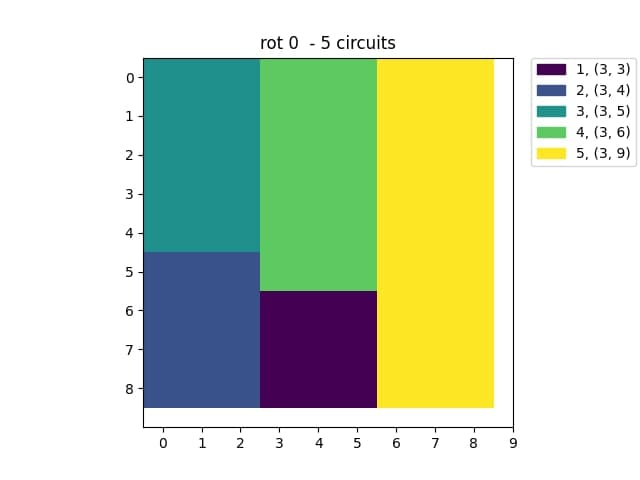
\includegraphics[width=2.5in]{images/sym_example/original.jpg} &
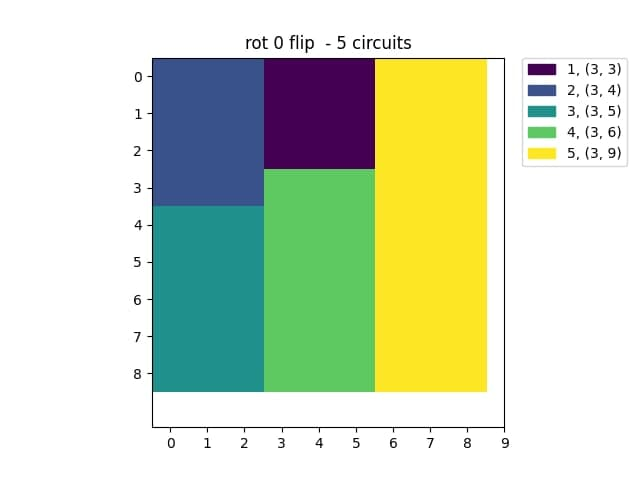
\includegraphics[width=2.5in]{images/sym_example/original_flipped.jpg} \\
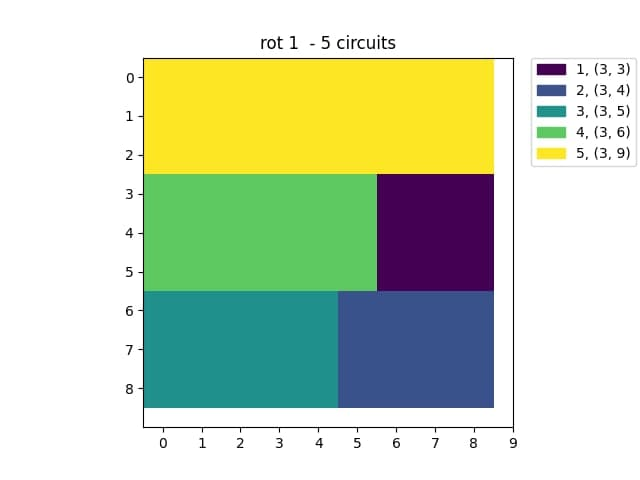
\includegraphics[width=2.5in]{images/sym_example/90.jpg} &
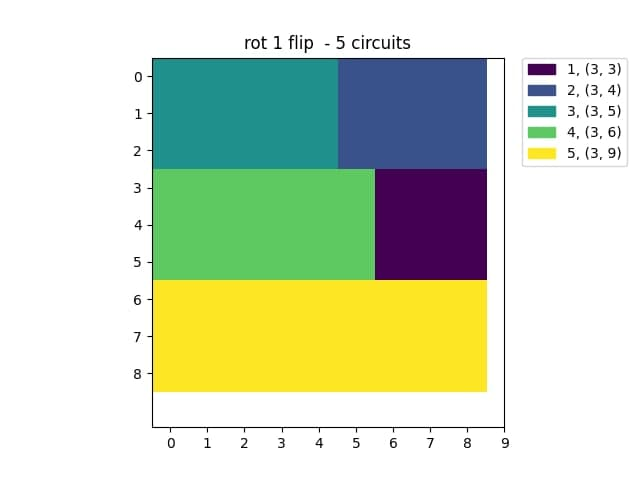
\includegraphics[width=2.5in]{images/sym_example/90_flipped.jpg} \\
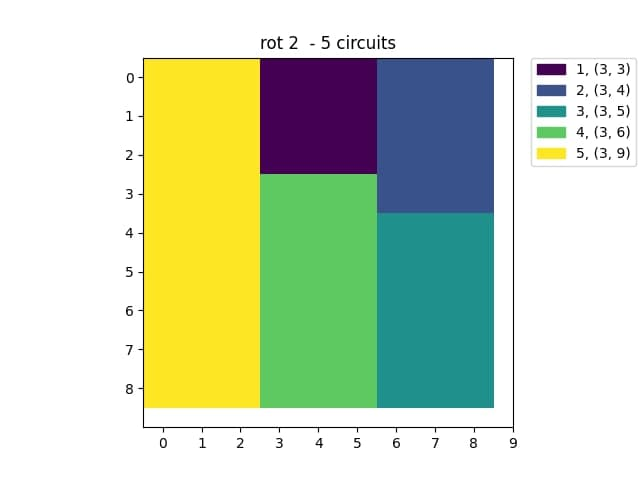
\includegraphics[width=2.5in]{images/sym_example/180.jpg} &
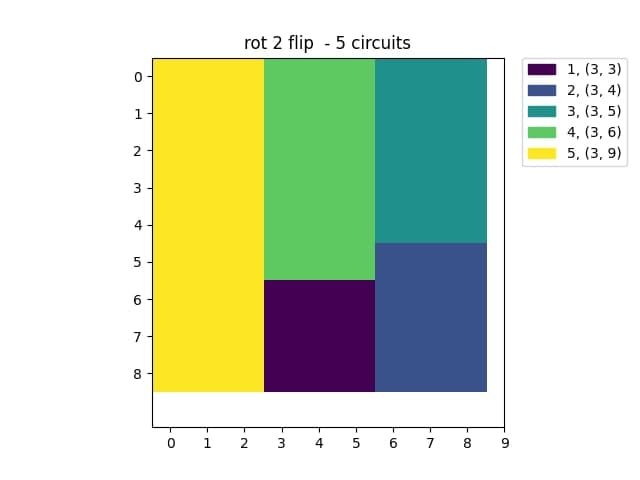
\includegraphics[width=2.5in]{images/sym_example/180_flipped.jpg} \\
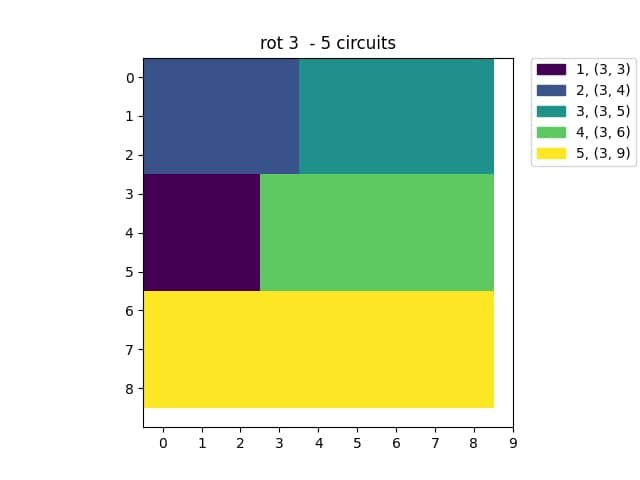
\includegraphics[width=2.5in]{images/sym_example/270.jpg} &
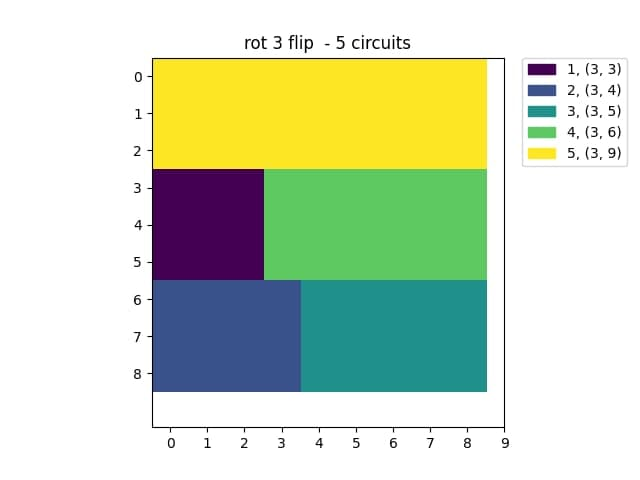
\includegraphics[width=2.5in]{images/sym_example/270_flipped.jpg} \\
\end{array}$
\end{center}
\caption{Second instance - all possible symmetric variants of a solution. Rot X indicates that the plate has undergone a rotation of X*90 degrees.}
\label{fig:symmetries}
\end{figure}

We could reduce the solver's work by reducing the number of solutions, thus by keeping only the non-symmetric ones. This can be done by placing the circuit with the largest area in the left-hand quarter of the silicon plate, namely by saying that $x_{big} \leq \dfrac{WIDTH}{2}$ and $y_{big} \leq \dfrac{HEIGHT}{2}$. This could be easily done in MiniZinc by adding this particular constraint:
\begin{lstlisting}[language=Mzn]
constraint symmetry_breaking_constraint(
    % This breaks the symmetries on the vertical axis
    corner_coords[biggest(), 1] * 2 <= width
    % This breaks the symmetries on the horizontal axis
    /\ corner_coords[biggest(), 2] * 2 <= height
    );
\end{lstlisting}
By looking at the figure \ref{fig:symmetries}, after the evaluation of the \textit{symmetry breaking constraint} the only solutions kept are 2 over the original 4, in the case we are not allowing rotation, whilst 4 over 8, in case of rotation.\\
A stronger \textit{symmetry breaking constraint} will place the biggest circuit in the lower-left corner of the silicon plate, namely in $(0,0)$:
$$x_{big} == 0 \land y_{big} == 0.$$
Nevertheless this constraint would not likely produce the desired effects, often slowing the solving process done by the MiniZinc's solver and as such it will not be considered in the CSP models comparison. The relative implementation is pretty straightforward:
\begin{lstlisting}[language=Mzn]
constraint symmetry_breaking_constraint(
    corner_coords[biggest(), 1] = 0
    /\ corner_coords[biggest(), 2] = 0
    );
\end{lstlisting}
\subsection{MiniZinc models comparisons}
The different models presented so far are now compared using a predefined configuration of the solver in order to avoid randomness in the results.
\\
\begin{table}[!h]
    \begin{tabular}{|c| p{2cm} | p{2 cm} | p{1.5cm} | c | c |}\hline
        Model &Rotation& Symmetry breaking& Solved instance & Mean time / instance (s) & Total time* (s) \\\hline
           1.0.0 & No  & No  & 23  & 30.79  & 708.20 \\ \hline
           1.3.0 & No  & No  & 25  & 6.86  & 171.56 \\ \hline
           1.0.0 & Yes & No  & 14  & 25.15 & 352.07 \\ \hline
           1.3.0 & Yes & No  & 17  & 43.59 & 741.02 \\ \hline
           1.0.0 & No  & Yes & 14  & 35.37  & 495.19 \\ \hline
           1.3.0 & No  & Yes & 22  & 21.19 & 466.13 \\ \hline
           1.0.0 & Yes & Yes & 21  & 26.32 & 552.82 \\ \hline
           1.3.0 & Yes & Yes & 26  & 17.48  & 454.53\\ \hline
    \end{tabular}
    \caption{MiniZinc models performances. Model 1.0.0 is the model without any global constraint, model 1.3.0 is the one with \texttt{diffn} and \texttt{cumulative}. (\emph{*}) the total time is computed by summing up successfully solved times.}
    \label{tab:csp-performance}
\end{table}

The best model is the \emph{1.3.0} the one with rotation and symmetry breaking, we think this is caused by the optimization done by the solver when we are using global constraints implemented in Minizinc. 
For further details, you can consult the file pdf \textbf{CSP\_performance.pdf}
\clearpage
    \section{Satisfiability modulo theories - SMT}
In computer science and mathematical logic, the \textbf{SMT} problem is a decision problem for logical formulas with respect to combinations of background theories expressed in \textbf{FOL}.\\
SMT can be thought of as a form of the constraint satisfaction problem and thus a certain formalized approach to constraint programming. \\

\subsection{SMT implementation}
To implement models in \textbf{SMT} we will use the library \textbf{Z3} in python notebooks.
\subsubsection{Without rotation}
To implement the model described in \hyperref[subsubsec:base-without-rot]{model without rotation} we used as variables: 
\begin{itemize}
    \item \textbf{x} to represent the X coordinates of the circuit;
    \item \textbf{y} to represent the Y coordinates of the circuit;
    \item \textbf{Height} to represent the maximum height reached by the circuits;
\end{itemize}
And as parameters we have:
\begin{itemize}
    \item \textbf{$N$} which represent the number of circuit;
    \item \textbf{$S$} to represent the set of circuit from 0\dots N;
    \item \textbf{$w_i$} to represent the width of circuit i;
    \item \textbf{$h_i$} to represent the height of circuit i;
    \item \textbf{WIDTH} which represent the width of the plate;
\end{itemize}
Then we added to the solver the following conditions: 
\begin{align}
    &width\_boundaries \equiv \forall{i \in  S}.(x_i \geq 0  \wedge  x_i + w_i \leq \textit{WIDTH}),\\
    &height\_boundaries \equiv \forall{i \in  S}.(y_i \geq 0  \wedge  y_i + h_i \leq \textit{HEIGHT}),
\end{align}
\begin{align}
   & no\_overlap\_cons \equiv \forall (i, j \in  S \text{ where } i \neq j).(\\
    &( x_i + w_i \leq x_j) \: \lor \\
    &( x_i - w_j \geq x_j) \: \lor \\
    &( y_i + h_i \leq y_j) \: \lor \\
    &(y_i - h_j \geq y_j)).
\end{align}
Hence, as the conjunction of all constraints we'll have: 
\begin{align}
    all\_constraints \equiv width\_boundaries \wedge height\_boundaries \wedge no\_overlap\_cons
\end{align}
Finally, by minimizing the \textbf{HEIGHT} we are reducing the empty area created by placing the circuits in the plate as the sum of area of the circuit is constant, although the \textbf{WIDTH} is fixed. 

\subsubsection{With rotation}
For the version of the model considering also the rotation, based on the previous model, we added a list of binary variables, which domain is defined as: 
\begin{equation}
    rot\_domain \equiv \forall{i \in S}.( rot_i \geq 0 \wedge  rot_i \leq 1)
\end{equation}
And we are considering the fact that: 
\begin{itemize}
    \item $rot_i$ is equal to 0, then the circuit $i$ is not rotated;
    \item $rot_i$ is equal to 1, then circuit $i$ is rotated by 90$^{\circ}$;
\end{itemize}
Then, we slightly modified constraints of the no rotation version as follows: 
\begin{align}
   & width\_boundaries \equiv \forall{i \in  S}.(x_i \geq 0  \wedge  x_i +(1-rot_i) w_i+ rot_i h_i \leq \textit{WIDTH})\\
    &height\_boundaries \equiv \forall{i \in  S}.(y_i \geq 0  \wedge  y_i + (1-rot_i)h_i + rot_i w_i \leq \textit{HEIGHT})
\end{align}
We simply considered that if a certain circuit $i$ is rotated, the $w_i$ and $h_i$ will be exchanged, so to compute the coordinates of the opposite corner, we will have to do the same.
\begin{align}
    &no\_overlap\_cons \equiv \forall (i, j \in  S \text{ where } i \neq j).(\\
      &(x_i + rot_i * h_i + (1 - rot_i) * w_i <= x_j) \: \\
     &\lor(y_i + rot_i * w_i + (1 - rot_i) * h_i <= y_j) \: \\
     &\lor(x_i - rot_j * h_j - (1 - rot_j) * w_j >= x_j) \: \\
     &\lor(y_i - rot_j * w_j - (1 - rot_j) * h_j >= y_j)\:
\end{align}
Also in this model, we set a objective function, the $height$, and our aim is to minimize it.

\subsection{Symmetry breaking}\label{subsec:smt-symmetry-breaking}
There are two symmetry breaking conditions, the first one is composed by the following:
\begin{equation}
    x_{big} * 2 \leq width \wedge y_{big}* 2\leq height
\end{equation}
In this case, we are forcing the biggest circuit to be placed in the a quadrant of the plate: 
\begin{figure}[!h]
 \centering
 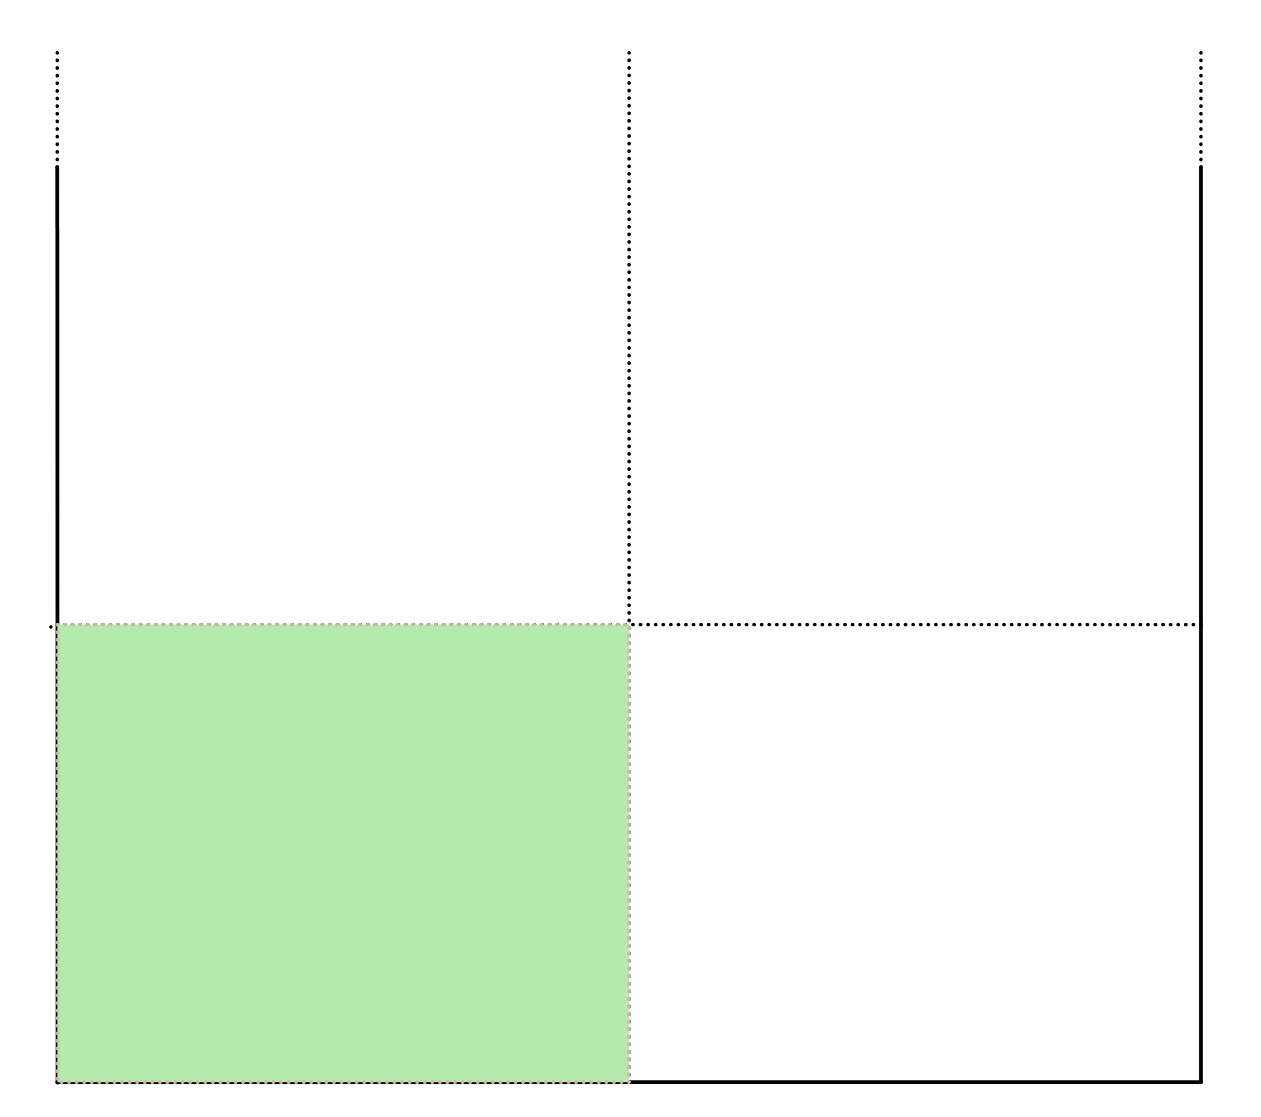
\includegraphics[width=12cm, height=8cm]{images/quadtants.PNG}
 \caption{Green area is the possible position of the biggest circuit}
\end{figure}\\
Meanwhile, the second one is the extreme case of the previous one, because we are imposing these conditions:
\begin{equation}
    x_{big} == 0 \wedge y_{big} == 0
\end{equation}
where $biggest$ is the index of the circuit with the biggest area. And in this case, the biggest circuit will be placed in the lower-left corner of the plate. Differently from what has been done with the MiniZinc implementation, here both of the symmetry constraints will be kept since the extreme case seems to perform better overall.  

\subsection{SMT models comparisons}
Now, we are going show the performance of different models over the 40 instances: \\
\begin{table}[!h]
    \begin{tabular}{|c| p{2cm} | p{2 cm} | p{1.5cm} | p{3.5cm} | c |}\hline
        Model &Rotation& Symmetry breaking& Solved instance & Mean time( solved instances) (s) & total time (s) \\\hline
           A &No  & No  & 22  & 16.78 & 369.11 \\ \hline
           B &No  & Yes & 24  & 29.51 & 708.27 \\ \hline
           C &Yes & No  & 14  & 38.94 & 545.23 \\ \hline
           D &Yes & Yes & 14  & 60.00 & 840.03 \\ \hline
    \end{tabular}
    \caption{SMT model performances}
    \label{tab:smt-performance}
\end{table}
\\
We can notice from the table that the model B has solved two instances in more w.r.t. the model A (instance 19 and 28 respectively with 242.95s and 180.94s), and because of this, it's mean time is higher than the one of A. 
\subsubsection{No rotation vs rotation}

From the previous table, we can notice a clearly improvement of the performance between model without rotation and the one with rotation, this is because in the latter one we have to consider when pieces are rotated, and the combination is $2^N$ times in more w.r.t. first one. 
\subsubsection{Two cases of symmetry breaking}

As we said in the \hyperref[subsec:smt-symmetry-breaking]{\S 4.2} there are two cases of symmetry breaking, the following table shows the different of performance when executing the models for instances from 10 to 19 as they are those more difficult to solve. We will only consider the model with rotation.

% Please add the following required packages to your document preamble:
% \usepackage[table,xcdraw]{xcolor}
% \documentclass[xcolor=table]{beamer}
% If you use beamer only pass "xcolor=table" option, i.e. 
\begin{table}[!h]
    \centering
    \begin{tabular}{|l|l|l|}
        \hline
         & Normal case & Extreme Case \\ \hline
        Instances 10 & 149.46      & 108.86       \\ \hline
        Instances 11 & 0.00         & 0.00          \\ \hline
        Instances 12 & 6.18        & 29.22        \\ \hline
        Instances 13 & 151.64      & 101.55       \\ \hline
        Instances 14 & 0.00         & 162.97       \\ \hline
        Instances 15 & 17.47       & 130.00       \\ \hline
        Instances 16 & 0.00         & 0.00          \\ \hline
        Instances 17 & 227.20      & 46.30        \\ \hline
        Instances 18 & 0.00         & 250.02       \\ \hline
        Instances 19 & 0.00         & 0.00          \\ \hline
        Solved instances & 5           & 7            \\ \hline
        Mean (All instances) & 205.1956    & 172.8912     \\ \hline
        Mean (Solved instances) & 110.40    & 118.42     \\ \hline
        Total time       & 2051.956    & 1728.912     \\ \hline
    \end{tabular}
    \caption{Execution statistics of instances 10 to 19.}
    \label{tab:my-table}
\end{table}
For the instances which are not solved within 300s, we abort the execution and consider the execution time as 0s. \\
The extreme case can solve 2 more instances w.r.t. the normal one, and if we recompute the mean time for extreme case, considering only instances solved by the normal case, the result would be \emph{83.19}, which is much lower than the normal case. 

\begin{figure}[!h]
 \centering
 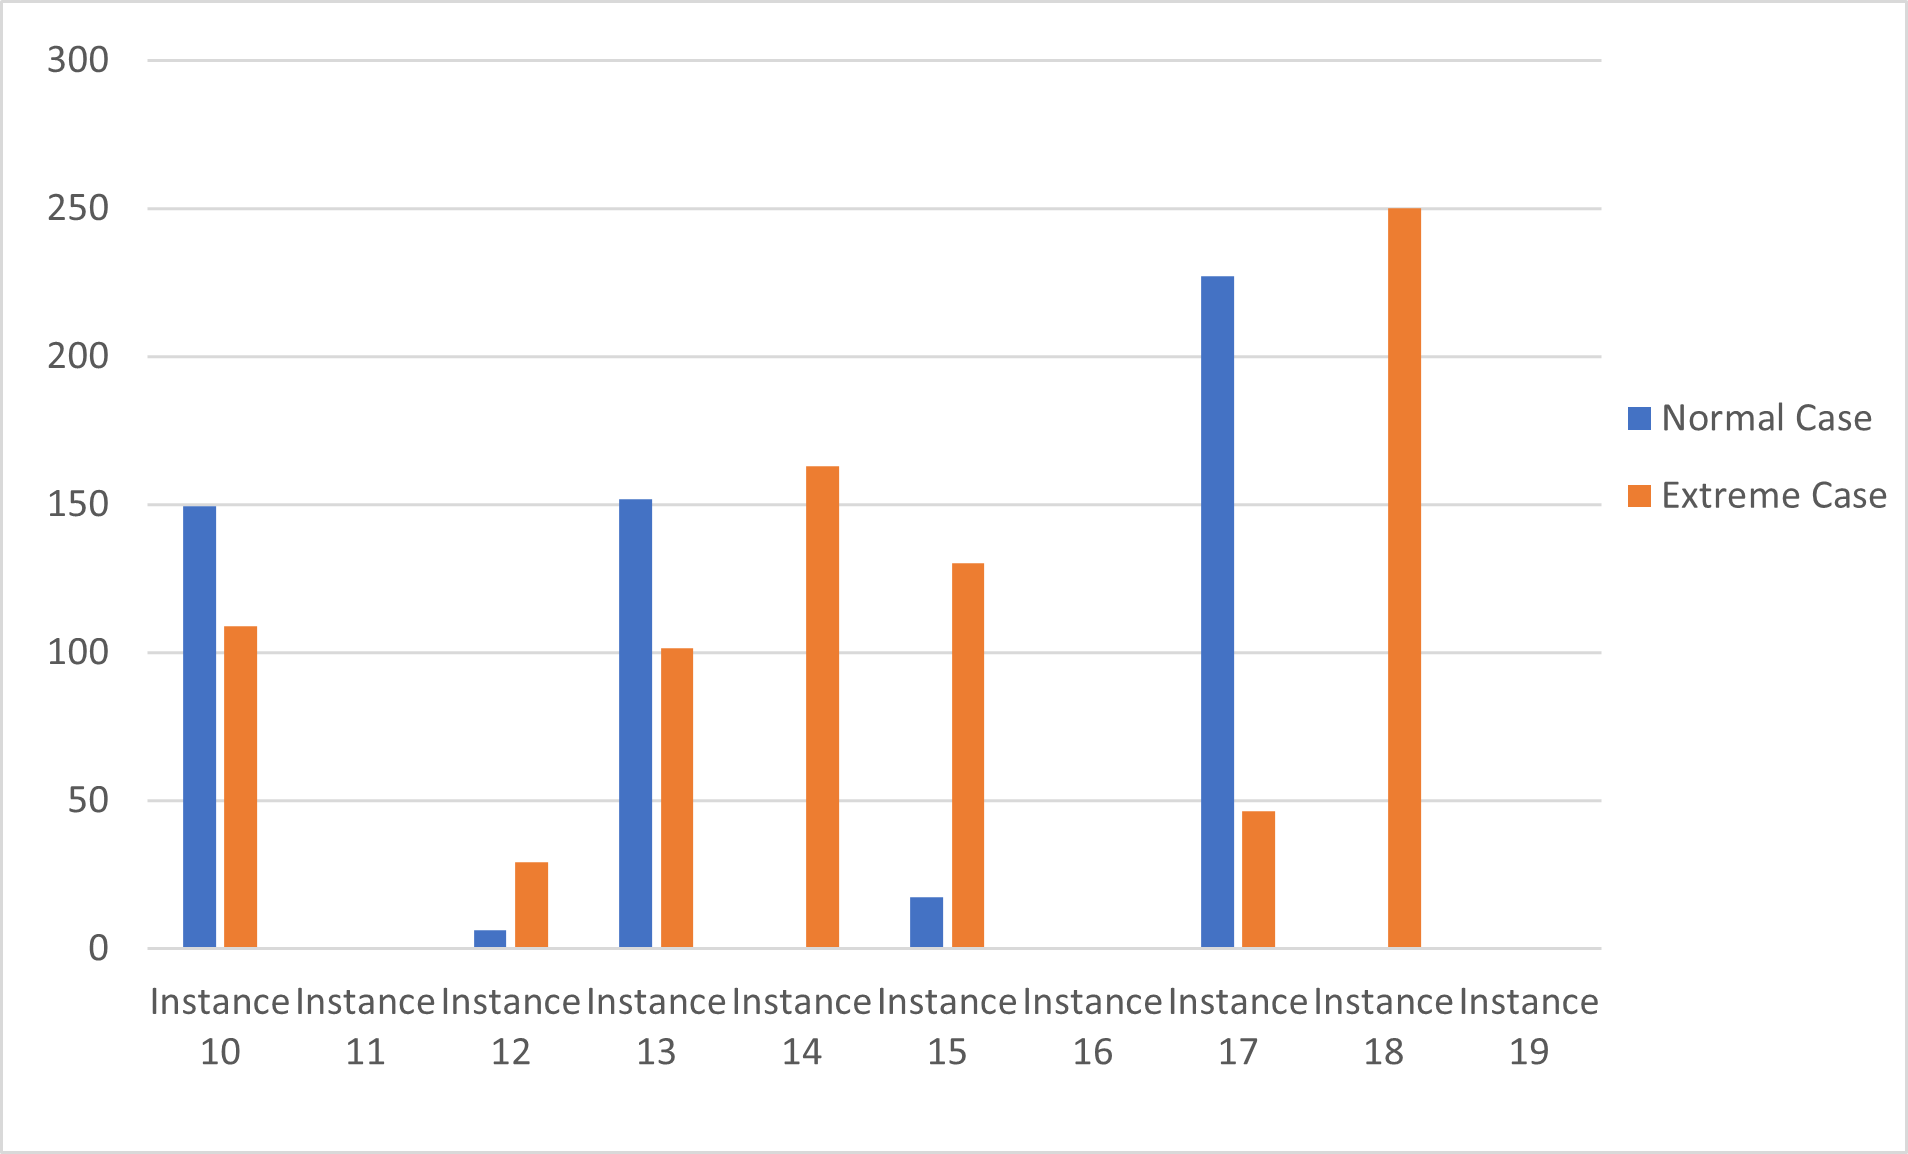
\includegraphics[width=14cm, height=10cm]{images/sym_breaking_smt_comparison.png}
 \caption{Symmetry breaking comparison.}
 \label{fig:sym-breaking-comparison}
\end{figure}

What we can see from the \hyperref[fig:sym-breaking-comparison]{graph} is that the extreme case works better.\\

Differently from the \textbf{CSP}, we can see a improvement of the performance of the extreme case of symmetry breaking. 

\clearpage
    \section{Results analysis and comparison}
In the following tables, we are going to compare the different versions of the model solving the instances from 10 to 19. When the instance is not successfully solved within 300 seconds, we set the time to \emph{0.00}. 
Compared versions are: 
\begin{itemize}
    \item \emph{CSP 1.0.0}: the base version of the model with only strictly needed constraints;
    \item \emph{CSP 1.3.0}: the version of the model with global constraints \emph{diffn} and \emph{cumulative};
    \item \emph{SMT}: the same as CSP 1.0.0 but implemented in SMT. 
\end{itemize}
\subsection{CSP vs SMT}
\begin{table}[!h]
    \centering
    \begin{tabular}{|c|c|c|c|}\hline
        Instances               & CSP 1.0.0  & CSP 1.3.0  & SMT      \\ \hline
        Instance 10             & 0.36   & 0.61   &   0.55  \\ \hline
        Instance 11             & 0.00   & 55.84  &   0.00  \\ \hline
        Instance 12             & 0.98   & 0.63   &   2.68  \\ \hline
        Instance 13             & 0.89   & 0.70   &   2.36  \\ \hline
        Instance 14             & 3.01   & 0.94   &   7.61  \\ \hline
        Instance 15             & 0.45   & 0.76   &   3.79  \\ \hline
        Instance 16             & 0.00   & 0.00   &   0.00  \\ \hline
        Instance 17             & 11.80  & 1.26   &   32.52 \\ \hline
        Instance 18             & 0.85   & 1.11   &   16.85 \\ \hline
        Instance 19             & 0.00   & 0.00   &   0.00  \\ \hline
        Solved   instances      & 7      & 8      & 7        \\ \hline
        Average   Solved(s)       & 2.62   & 7.73   & 9.48     \\ \hline
        % Model Execution(s)    & 920.15 & 666.14 & 966.35   \\ \hline
        % Total Solved Instances(s) & 20.15  & 66.14  & 66.35    \\ \hline
    \end{tabular}
    \caption{CSP VS SMT base}
    \label{tab:csp-smt-base-comparison}
\end{table}
In this comparison, we can notice that \textbf{CSP 1.3.0} works better than others, because it can solve the instance 11, although it takes \textit{55.84} seconds. If we recompute the average solved time not considering instance 11, we would obtain as mean time \textit{0.75} second per instance.

\subsection{CSP vs SMT with symmetry breaking}
% modelli CSP con rotazione e SMT con symmetry breaking (Si)
\begin{table}[!h]
    \centering
    \begin{tabular}{|c|c|c|c|}\hline
        Instances               & CSP 1.0.0  & CSP 1.3.0   & SMT    \\ \hline
        Instance 10             & 1.05   & 0.41    & 0.47   \\ \hline
        Instance 11             & 0.00   & 42.41  & 0.00   \\ \hline
        Instance 12             & 1.11   & 0.48    & 1.54   \\ \hline
        Instance 13             & 1.09   & 0.52    & 1.55   \\ \hline
        Instance 14             & 1.59   & 0.74    & 2.49   \\ \hline
        Instance 15             & 1.97   & 0.79    & 1.97   \\ \hline
        Instance 16             & 0.00   & 0.00  & 0.00   \\ \hline
        Instance 17             & 7.52   & 1.11    & 37.29  \\ \hline
        Instance 18             & 99.53   & 2.12   & 11.34  \\ \hline
        Instance 19             & 0.00   & 0.00    & 0.00   \\ \hline
        Solved   instances      & 7      & 8       & 7      \\ \hline
        Average   Solved(s)        & 16.27   & 6.07   & 8.09   \\ \hline
        % Model Execution(s)    & 915.22 & 1647.11 & 956.66 \\ \hline
        % Solved   Instances(s) & 15.22  & 147.11  & 56.66  \\ \hline
    \end{tabular}
    \caption{CSP VS SMT with symmetry breaking}
    \label{tab:csp-smt-with-symm-comparison}
\end{table}
In this version of the model, we can notice that \textbf{CSP 1.3.0} can solve the \textit{instance 11} which is not solved by other models. For other instances, we can see that \textbf{CSP 1.3.0} can solve them in quite similar time w.r.t. other models.\\



\subsection{CSP vs SMT with rotation}
% modelli CSP con rotazione e SMT con rotazione (No)

\begin{table}[!h]
    \centering
    \begin{tabular}{|c|c|c|c|}\hline
        Instances               & 1.0.0  & 1.3.0  & SMT    \\ \hline
        Instance 10             & 26.05  & 0.50   & 206.93 \\ \hline
        Instance 11             & 0.00   & 150.08 & 0.00   \\ \hline
        Instance 12             & 0.00   & 1.44   & 4.55   \\ \hline
        Instance 13             & 19.52  & 0.88   & 0.00   \\ \hline
        Instance 14             & 264.99 & 72.59  & 0.00   \\ \hline
        Instance 15             & 1.05   & 32.46  & 36.76  \\ \hline
        Instance 16             & 0.00   & 0.00   & 0.00   \\ \hline
        Instance 17             & 0.00   & 187.57 & 0.00   \\ \hline
        Instance 18             & 0.00   & 0.00   & 61.27  \\ \hline
        Instance 19             & 0.00   & 0.00   & 0.00   \\ \hline
        Solved   instances      &  4     &       &       \\ \hline
        Average   Solved        &  77.90   &  63.65   &  77.38   \\ \hline
    \end{tabular}
    \caption{CSP VS SMT with rotations}
    \label{tab:csp-smt-with-rot-comparison}
\end{table}
In the models with rotation, we can expect that the solving time are longer than the model without rotations, because we need to consider more variables.
So, with the timeout of 300 seconds, we can solve less instances. 
Also in this comparison, we can see that the \textbf{CSP 1.3.0} works better, still, this could be caused by the optimizations done by the solver with global constraints. \\
\subsection{CSP vs SMT with symmetry breaking and rotation}
% modelli CSP con rot e sym vs SMT rot e sym (Si)

\begin{table}[!h]
    \centering
    \begin{tabular}{|c|c|c|c|}\hline
        Instances          & 1.0.0    & 1.3.0    & SMT  \\ \hline
        Instance 10        & 61.74    & 0.44     & 121.9323  \\ \hline
        Instance 11        & 0.00     & 133.78   & 0    \\ \hline
        Instance 12        & 135.53   & 0.81     & 154.3911  \\ \hline
        Instance 13        & 13.36    & 0.65     & 279.6322  \\ \hline
        Instance 14        & 0.00     & 1.16     & 212.5075  \\ \hline
        Instance 15        & 31.92    & 0.78     & 61.53585  \\ \hline
        Instance 16        & 0.00     & 0.00     & 0    \\ \hline
        Instance 17        & 0.00     & 2.20     & 0    \\ \hline
        Instance 18        & 0.00     & 5.74     & 0    \\ \hline
        Instance 19        & 0.00     & 0.00     & 0    \\ \hline
        Solved   instances &  4  &  8 &  5  \\ \hline
        Average   Solved   &  60.64 &  18.19 &  166.00 \\ \hline
        % Model Execution time    & 1630.06 & 652.55 & 2330.00 \\ \hline
        % Solved   Instances(s) & 130.06  & 52.55  & 830.00  \\ \hline
    \end{tabular}
    \caption{CSP VS SMT with rotation and symmetry breaking}
    \label{tab:csp-smt-with-rot-sym-comparison}
\end{table}
By combining the previous two cases, we can produce a model which is able to solve \textit{8} instances, with average time \textit{6.57}s. But still, other two models work worse than the \textbf{CSP 1.3.0}, this can be caused by the use of the global constraints. \\
Considering also the fact that the computational power required to satisfy symmetry breaking constraints and rotations is much higher. 
\clearpage
    \section{Conclusion and future developments}
\subsection{Possible future developments}
%  possibile introdure altri symmetry breaking
One of possible future development is to introduce new symmetry breaking as follows: once we have found a solution, we can represent it as a bi-dimensional matrix $M$, in which every value $M_{i,j} \in \{0,\dots,N\}$, then it is possible to encode each circuit as a sub-matrix of $M$, such that for a generic circuit $v$, $M_{x_{v} \dots w_v, y_v \dots h_v} = v$. A possible example, representing the solution of figure \ref{fig:future}, is the following:
\begin{center}
    $ \begin{bmatrix}
        1 & 1 & 1 & 3 & 3 & 3 & 3 & 3 \\
        1 & 1 & 1 & 3 & 3 & 3 & 3 & 3 \\
        1 & 1 & 1 & 3 & 3 & 3 & 3 & 3 \\
        4 & 4 & 4 & 4 & 4 & 2 & 2 & 2  \\
        4 & 4 & 4 & 4 & 4 & 2 & 2 & 2  \\
        4 & 4 & 4 & 4 & 4 & 2 & 2 & 2  \\
        4 & 4 & 4 & 4 & 4 & 2 & 2 & 2  \\
        4 & 4 & 4 & 4 & 4 & 2 & 2 & 2
    \end{bmatrix}  $
    \label{Solution as Matrix}
\end{center}

In order to reduce the number of symmetries to be computed by the solver we can impose an ordering between the matrix $M$ and other possible permutation of it. In particular we can state that:
\begin{itemize}
    \item to remove the original version flipped vertically:
        \begin{equation*}
            \text{lex\_lesseq}(\text{array1d(M)}, M[i, j] \text{ where } i \in \{HEIGHT,\dots,1\}, j \in \{1, \dots, WIDTH\});
        \end{equation*}
    \item to remove the rotated version by 180°:
        \begin{equation*}
            \text{lex\_lesseq}(\text{array1d(M)}, M[i, j] \text{ where } i \in \{HEIGHT,\dots,1\}, j \in \{WIDTH, \dots, 1\});
        \end{equation*}
    \item to remove the 180 degrees rotated and flipped vertically version:
        \begin{equation*}
            \text{lex\_lesseq}(\text{array1d(M)}, M[i, j] \text{ where } i \in \{1,\dots,HEIGHT\}, j \in \{WIDTH, \dots, 1\}).
        \end{equation*}
\end{itemize}

\begin{figure}[!h]
 \centering
 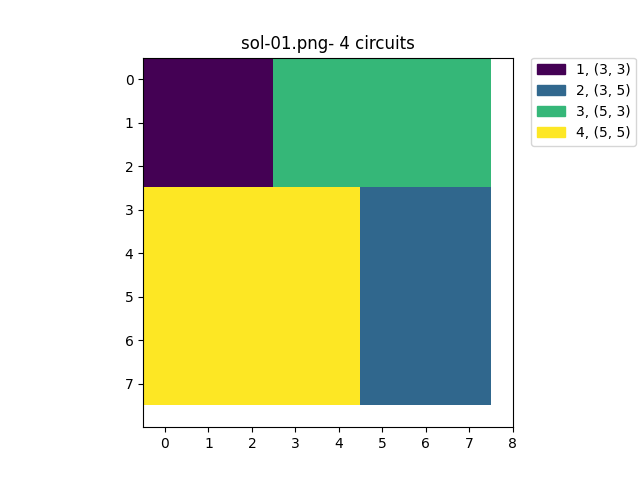
\includegraphics[width=12cm, height=10cm]{images/sol-01.png}
 \caption{Solution as image}
 \label{fig:future}
\end{figure}

\subsection{Final considerations}
By developing this project, many theoretical concepts are clarified and applied in a practical way. \\
As first step, we reasoned on how to model a problem identifying which are parameters and variables, how to encode it in different languages, such as Minizinc and SMT, then we tried to improve the model by introducing in Minizinc global constraints, implied constraints or conditions, and finally symmetry breaking constraints. We though that this procedure is much efficient. \\
Then, we did different experiments by changing configuration parameters, for Minizinc models, we found that the fastest way to find the correct solution is to apply \emph{first\_fail} as the criteria to choose the variable, and \emph{indomain\_min} to choose the value.\\

We can say that \textbf{CSP 1.3.0} seems to perform better than \textbf{SMT} and \textbf{CSP 1.0.0}, at least it should asymptotically do so. Below we have summarized some datum about the model mentioned on the \textbf{40} instances given as reference:
\begin{itemize}
    \item \textbf{Solved instances}: \textit{26};
    \item \textbf{Average solving time}: \textit{17.48s};
    \item \textbf{Total execution time for the solved instances}: \textit{454.53s}
\end{itemize}
\clearpage
	\nocite{*} % Flag to put all citations in the bibliography
	\printbibliography
\end{document}
